\documentclass[../template]{subfiles}

\begin{document}
\section{RTL in regione dinamica}
\begin{minipage}{.4\textwidth}
    \begin{center}
        \begin{circuitikz}
            \draw (0, 0)
            node[ground]{}
            node[npn, anchor=E] (npn){}

            (npn.B) to[R] ++(-1.5, 0)
            node[circ]{} node[above]{$V_i$}

            (npn.C) to[R] ++ (0, 1.5)
            node[vcc]{}

            (npn.C) -- ++(.2, 0) node[circ]{} node[right]{$V_u$}

            ;
    \end{circuitikz}
\end{center}
\end{minipage}
\begin{minipage}{.5\textwidth}
    \begin{center}
        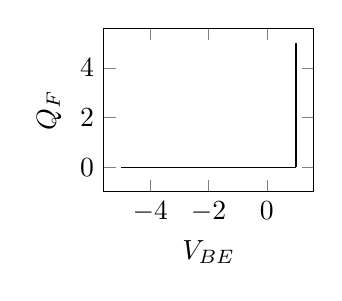
\begin{tikzpicture}
            \begin{axis}[ylabel=$Q_F$, xlabel=$V_{BE}$, ymin=-1, width=.35\textwidth]
                \addplot[domain=-5:1, black] {0};
                \addplot[black] coordinates {(1, 0) (1, 5)};
            \end{axis}
        \end{tikzpicture}
        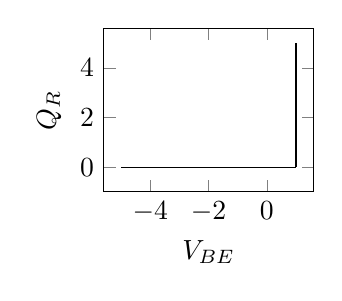
\begin{tikzpicture}
            \begin{axis}[ylabel=$Q_R$, ymin=-1, xlabel=$V_{BE}$, width=.35\textwidth]
                \addplot[black, domain=-5:1] {0};
                \addplot[black] coordinates {(1, 0) (1, 5)};
            \end{axis}
        \end{tikzpicture}
    \end{center}

    \begin{center}
        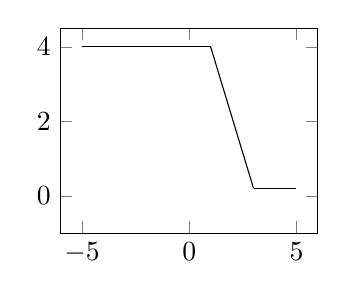
\begin{tikzpicture}
            \begin{axis}[width=.4\textwidth, ymin=-1]
                \addplot[black, domain=-5:1] {4};
                \addplot[black, domain=1:3] coordinates {(1, 4) (3, 0.2)};
                \addplot[black, domain=3: 5] {0.2};
            \end{axis}
        \end{tikzpicture}
    \end{center}
\end{minipage}

Ricordandoci i modelli di approssimazione utilizzati, descritti dalle equazioni:
\[
    Q_F \coloneqq
    \begin{cases}
        Q_+ = 0 &\text{per} \quad V_{BE} < V_\gamma
        \\
        V_{BE} = V_\gamma &\text{per} \quad Q_F > 0
    \end{cases}
\]
\[
    Q_R \coloneqq
    \begin{cases}
        V_{BC} = V_\gamma' & \text{per} \quad  Q_R > 0\\
        Q_R = 0 & \text{per} \quad V_{BC} < V_\gamma'
    \end{cases}
\]
Ricordiamo inoltre che $V_\gamma - V_\gamma' = \vcesat$ quando entrambe le giunzioni sono polarizzate in diretta. E l'uscita si porta al valore alto quando il transistore è spento, ed il valore basso quando è in saturazione.

Tenendo presente questi dati calcoliamo il comportamento del circuito in regime dinamico, presupponendo un'ingresso a gradino, dove
\[
    V_i(t) =
    \begin{cases}
        0 & \text{per} \quad t < 0 \\
        V_{cc} & \text{per} \quad t > 0
    \end{cases}
\]
\begin{tcolorbox}
    Per $t < 0$, siccome siamo in regioni statiche conosciamo già il valore dell'uscita: $V_u = V_{cc}$.
    Quindi, sapendo che il transistore è spento, $I_B = 0$, e $V_i = V_{BE} = 0$.
    Guardando in corrispondenza del grafico il valore della carica: $Q_F = 0$

    Siccome $V_{BC} = V_{BE} - V_{cc} = -V_{cc}$, allora $Q_R = 0$
\end{tcolorbox}
\begin{tcolorbox}
    Per $t \to \infty$ il transistore si trova in regione di saturazione, quindi $V_u = \vcesat$, ed essendo $V_{BE} = V_\gamma$, allora $Q_F > 0$ e $V_{BC} = V_\gamma'$ quindi $Q_R > 0$.

    \begin{align*}
        &I_B = \frac{V_{cc} - V_\gamma}{R_B} = \frac{Q_F}{\beta_F \tau_F} + \frac{Q_R}{\beta_B \tau_R}
        \\
        &I_C = \frac{V_{cc} - \vcesat}{R_C} = \frac{Q_F}{\tau_F} - \frac{Q_R}{\alpha_R \tau_R}
    \end{align*}

    Da cui, indicando con $\frac{1}{M} \frac{1}{\tau_R} \big( \frac{1}{\alpha_R} + \frac{\beta_F}{\beta_R}\big)$ si può scrivere:
    \[
        Q_R = M (\frac{\beta_F(V_{cc} - V_\gamma)}{R_B} - \frac{(V_{cc} - \vcesat)}{R_C})
    \]
    \[
        \frac{Q_F}{tau_F} = \frac{V_{cc} - \vcesat}{R_C} + \frac{Q_R}{\alpha_R \tau_R}
    \]

    Siccome la carica $Q_R$ deve esser positiva, allora controllando la condizione, si ottiene:
    \[
        \vcesat < V_{cc} - \frac{\beta_F R_C}{R_B} (V_{cc} - V_\gamma)
    \]
    dove la condizione a destra della disuguaglianza è il tratto obliquo della retta del grafico di $V_u(V_i)$, tanto più la condizione è verificata, tento più è maggiore la carica $Q_R$ associata al transistore e maggiore è la durata del transitorio.
    Diminuire la carica va quindi in conflitto con l'obbiettivo di diminuire il margine ai ritardi del transitorio.
\end{tcolorbox}

Ovviamente, nel transitorio della carica da $Q =0$ a $Q$ verticale, (vedi grafico carica) sarà necessario passare in un punto intermedio ($C$).
% 34:39
\begin{tcolorbox}
    \begin{align*}
        V_{BC} = V_{BE} - V_{CE}
        \\
        V_{BC} = V_\gamma - V_{cc}
    \end{align*}

\end{tcolorbox}
Descriviamo quindi il transitorio da $A$ a $B$, separandolo in due intervalli:
Un primo tratto, da $A$ a $C$, dove sono vere le equazioni:
\begin{align*}
    Q_F = 0 \\
    Q_R = 0 \\
    V_{BE} < V_\gamma \\
    V_{BC} < V_\gamma'
\end{align*}

Un secondo tratto da $C$ a $D$:
\begin{align*}
    Q_F > 0 \\
    Q_R = 0 \\
    V_{BE} = V_\gamma \\
    V_{BC} < V_\gamma'
\end{align*}

Ed un terzo tratto da $D$ a $B$:
\begin{align*}
    &Q_F > 0 \\
    &Q_R > 0 \\
    &\begin{rcases}
        V_{BE} = V_\gamma \\
        V_{BC} > V_\gamma '
    \end{rcases} \Rightarrow V_{CE} = \vcesat
\end{align*}

\subsubsection{Analisi dei tratti della caratteristica}
Nel primo tratto, non essendoci spostamento di carica il transitorio è istantaneo.  In un tempo potenzialmente nullo, la tensione $V_{BE}$, raggiunge il valore di $V_\gamma$.

Nel secondo tratto, necessariamente la corrente $I_B = \frac{Q_F}{\beta_F \tau_F} + \frac{Q_R}{\beta_R \tau_R} + \frac{dQ_F}{dt} + \frac{dQ_R}{dt}$, siccome la carica $Q_R$ è nulla, allora viene espressa come:
\[
    I_B = \frac{Q_F}{\beta_F \tau_F} + \frac{dQ_F}{dt}
\]
Inoltre, dall'equazione di kirkoff, sappiamo che $I_B = \frac{V_u - V_\gamma}{R_B}$.
Dall'equazione della carica $I_B$ precedente possiamo scrivere:
\[
    \frac{dQ_F}{dt} = I_B - \frac{Q_F}{\beta_F \tau_F} =  - \frac{1}{\beta_F \tau_F} (Q_F - M)
\]
Ed integrando si ottiene:
\[
    \ln \frac{Q_F(t) - M}{- M} = - \frac{t} {\beta_F \tau_F}
\]

Da cui:
\[
    Q_F(t) = M(1 - e^{-\frac{t}{\beta_F \tau_F}}) = \frac{\beta_F \tau_F (V_{cc} - V_\gamma)}{R_B} (1 - e^{-\frac{t}{\beta_F \tau_F}})
\]
Tutto questo è vero fino a quando non viene raggiunto il punto $D$, in cui $V_{BE} = V_\gamma$ e $V_{BC} = V_\gamma'$, quindi $V_{CE} = V_u = \vcesat$.
Scrivendo l'equazione di $V_{cc}$, otteniamo:

\[
    V_u = V_{cc} - R_C I_C = V_{cc} - \frac{\beta_F R_C}{R_B} (V_{cc} - V_\gamma) (1 - e ^ {-\frac{t}{beta_F \tau_F}})
\]


Analizzando il terzo tratto del transitorio, dove $V_{BE} = V_\gamma$, $V_{BC} = V_\gamma'$ e $Q_F, Q_R > 0$, facendo sempre riferimento
all'equazione della corrente $I_C$ ed $I_B$, dove questa volta tutte le componenti sono significative.

Inoltre siccome $V_{BE} V_\gamma$ e $V_{BC} = V_\gamma'$, l'uscita $V_u = V_{CE} = V_\gamma - V_\gamma' = \vcesat$. Unendo le equazioni delle due correnti quindi otteniamo il sistema:
\[\begin{cases}
    I_C = \frac{Q_F}{\tau_F} - \frac{Q_R}{\alpha_R \tau_R} - \frac{dQ_R}{dt} = \frac{V_{cc} - \vcesat}{R_C}
    \\
    I_B = \frac{Q_F}{\beta_F\tau_F} + \frac{Q_R}{\beta_R \tau_R} + \frac{dQ_R}{dt} + \frac{dQ_R}{dt}= \frac{V_{cc} - V_\gamma}{R_B}
\end{cases}\]
Siccome sappiamo già che l'uscita $V_u$ è costante ed indipendente dal tempo, la carica continua a crescere e sappiamo già a quali valori tende asintoticamente. Quindi dopo un tempo sufficientemente lungo abbiamo già calcolato il valore della caratteristica.

\subsubsection{Studio transitorio "gradino in discesa"}
Studiamo il transitorio percorrendo i punti da $B$ ad $A$.
Nel tratto iniziale, caratterizzato da $Q_F, Q_R > 0$ abbiamo $V_u = \vcesat$. Quando il valore di $Q_R$ raggiunge 0, allora il punto coincide con il punto $D$ della caratteristica. Esattamente come il diodo, esso prima di spegnersi mantiene ai suoi capi una tensione costante.
Calcolando nell'intervallo la corrente di base:
\[
    I_B = \frac{V_i = V_{BE}} {R_B} = -\frac{V_\gamma}{R_B}
\]
Una corrente negativa, che ricorda il tratto di spegnimento del diodo, in quanto stiamo passando dalla regione di saturazione, dove entrambe le giunzioni sono polarizzate in diretta, alla regione normale, dove la regione è polarizzata in inversa. Nell'intervallo anche la carica $Q_R$, varia secondo una relazione non ancora definita nel dettaglio, senza raggiungere 0.


Analizzando il secondo tratto del transitorio, da $D$ a $C$, caratterizzato da $V_{BE} = V_\gamma$, $V_{BC} < V_\gamma'$ di conseguenza $V_u > \vcesat$. $Q_F > 0$ e $Q_R = 0$. Possiamo quindi scrivere un'equazione simile a quella espressa in precedenza ricordando la formula della corrente:
\begin{align*}
    &I_B  = \frac{Q_F}{\beta_F I_F} + \frac{Q_R}{\beta_R \tau_R} + \frac{dQ_F}{dt} + \frac{dQ_R}{dt}
          =  \frac{Q_F}{\beta_F I_F} + \frac{dQ_F}{dt}  = -\frac{V_\gamma}{R_B}
    \\
    \frac{dQ_F}{dt} =
\end{align*}


\end{document}

